\documentclass{article}

\usepackage{geometry}
\geometry{
  a4paper,           % or letterpaper
  textwidth = 14cm,  % llncs has 12.2cm
  textheight = 21cm, % llncs has 19.3cm
  heightrounded,     % integer number of lines
  hratio = 1:1,      % horizontally centered
  vratio = 2:3,      % not vertically centered
}

\usepackage[utf8]{inputenc}
\usepackage[portuguese]{babel}
\usepackage{graphicx, color}
\usepackage{indentfirst}
\usepackage[hidelinks]{hyperref}
\usepackage[capposition=top]{floatrow}

\setlength{\parskip}{0.4cm}
\renewcommand{\baselinestretch}{1.1}

\begin{document}

\begin{titlepage}
	\centering
	\def\svgwidth{0.6\textwidth}
	\input{fcup_logo.eps_tex}\par
	\vspace{1cm}
	{\scshape\Large Sistemas Distribuídos\par}
	\vspace{3cm}
	{\Huge\bfseries Video Streaming\par}
	\vspace{5cm}
	{\Large\itshape Marco Pontes | Nuno Azevedo\par}
	\vspace{0.5cm}
	{\Large up201308000@fc.up.pt | up201306310@fc.up.pt\par}
	\vfill
	{\large \today}
\end{titlepage}

\newpage
\setcounter{page}{2}

\begin{abstract}
O objetivo deste projeto é a implementação de um serviço de \textit{streaming} de vídeo. A comunicação entre os vários 		elementos intervenientes assenta na tecnologia \textit{Ice}\footnote{\url{https://zeroc.com/products/ice}}.
\end{abstract}


\section{Introdução}

O \textit{Ice} é uma estrutura de comunicação entre processos (\textit{RPC framework}) que fornece vários conjuntos de ferramentas de desenvolvimento de software. Esta implementa um protocolo de comunicação próprio, \textit{Ice Protocol \footnote{\url{https://doc.zeroc.com/display/Ice36/Overview+of+the+Ice+Protocol}}}, que suporta tanto \textit{TCP/IP} como \textit{UDP} oferecendo assim uma comunicação funcional a aplicações através da internet. Este protocolo também permite usar o protocolo \textit{Secure Socket Layer (SSL)\footnote{\url{https://doc.zeroc.com/display/Ice36/IceSSL}}} oferecendo uma comunicação encriptada entre o cliente e o servidor. 

A estrutura pode ser usada em várias linguagens de programação como \textit{C++}, \textit{C\#}, \textit{Java}, \textit{Python}, entre outras. A linguagem escolhida para o desenvolvimento do serviço de \textit{streaming} de vídeo foi \textit{Java} devido ao conforto já adquirido com a linguagem.

O serviço de \textit{streaming} de vídeo é constituído por um Portal, um Cliente e um \textit{Streamer}. O \textit{Streamer} será o responsável por efetuar a \textit{streaming} de vídeo, o Cliente de receber e visualizar o vídeo e o Portal de realizar a gestão dos \textit{streamers} disponíveis e comunicar essas informações aos clientes.

\newpage


\section{Descrição}

Na figura seguinte é possível visualizar a interação entre os diferentes componentes:\\

%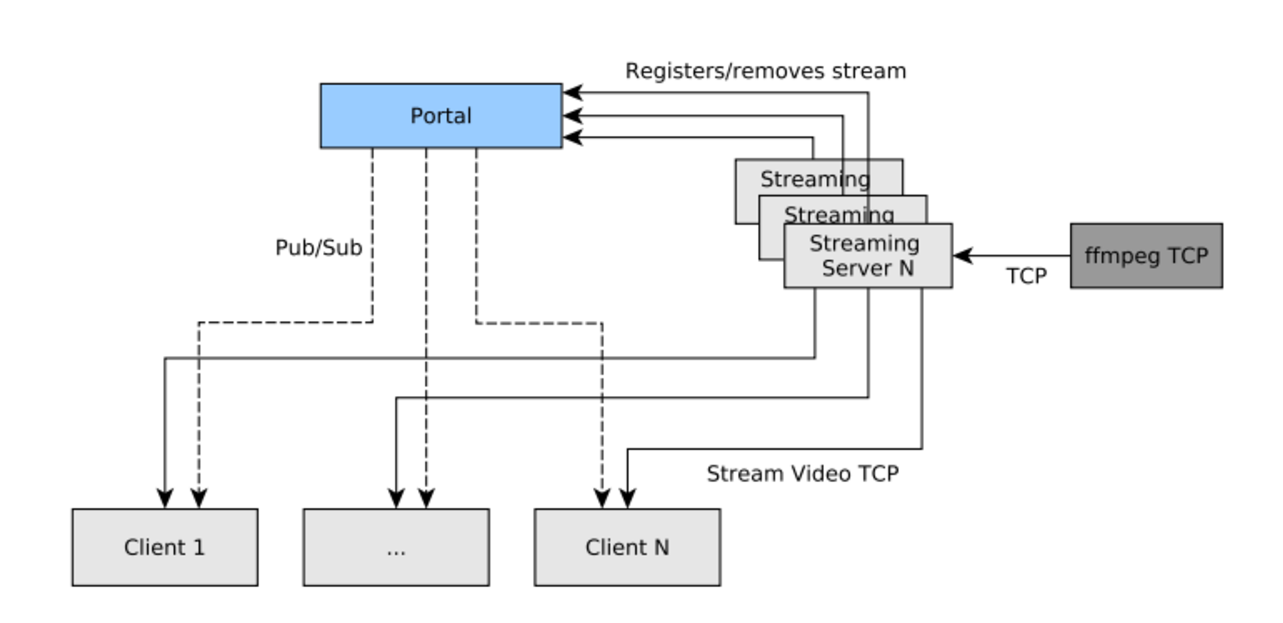
\includegraphics[scale=0.70]{scheme.eps}
\begin{figure}[h]
\def\svgwidth{1\textwidth\centering}
\input{scheme.eps_tex}
\caption{Interação entre os componentes.}
\floatfoot{\textit{Origem:} \url{http://www.dcc.fc.up.pt/~rmartins/aulas/sd1617/trabII/trabII.pdf}\vspace{0.3cm}}
\label{fig:scheme}
\end{figure}

Com base na figura \ref{fig:scheme}, temos as seguintes funções de cada componente:

\begin{itemize}

	\item \textbf{Portal:}
		\begin{itemize}
			\item Receber informações dos \textit{streaming servers}, permitindo o registo e remoção de servidores, realizando as comunicações através do \textit{Ice RPC};
			\item Informar todos os clientes dos \textit{streaming servers} existentes, também através do \textit{Ice RPC}; 
			\item Sempre que um novo \textit{Streamer} se registar ou terminar, o Portal informará todos os clientes desse evento. Esta comunicação é efetuada através do \textit{IceStorm\footnote{\url{https://zeroc.com/products/ice/services/icestorm}}}, um serviço de distribuição \textit{Publisher/Subscriber}.
		\end{itemize}
		
	\item \textbf{\textit{Streamer}:}
		\begin{itemize}
			\item Registar-se no Portal como um \textit{streaming server} com todas as suas informações:
			\begin{itemize}
				\item Nome da \textit{stream};
				\item Endereço da \textit{stream} constituído por tipo de protocolo, endereço IP e a porta;
				\item Resolução do vídeo;
				\item Velocidade de transmissão;
				\item Conjunto de tópicos que caracterizem o vídeo.
			\end{itemize}
			\item Ao encerrar o \textit{streaming server}, informa o Portal para que este atualize as suas informações.
			\item Transmite o vídeo usando o programa \textit{FFmpeg\footnote{\url{https://ffmpeg.org/}}} para um endereço. De seguida,  cria uma socket nesse endereço com o objetivo de ler o output do \textit{FFmpeg} para voltar a transmitir para outro endereço usando um \textit{ServerSocket} para que múltiplos clientes possam visualizar a \textit{stream}.
		\end{itemize}

	\item \textbf{Cliente:}
		\begin{itemize}
			\item Através do \textit{Ice RPC}, pedir ao Portal a lista de \textit{streams} existentes.
			\item Registar-se no serviço de \textit{Publisher} no Portal para passar a receber informações das novas \textit{streams} ou de \textit{streams} removidas.
			\item Reproduzir o conteúdo disponibilizado pelo \textit{streaming server} através do \textit{ffplay}.
		\end{itemize}
\end{itemize}


\subsection{Metodologia}

Para o desenvolvimento do projeto usamos o \textit{IDE IntelliJ IDEA}\footnote{\url{https://www.jetbrains.com/idea/}} de forma a tornar a programação mais rápida e eficiente, além de que nos ajudou imenso a conhecer os vários métodos disponíveis nas bibliotecas usadas durante o desenvolvimento do projeto.

Pela facilidade de trabalhar em grupo, de ter registos de toda a atividade do projeto, como também nos permitir ter o código guardado de forma segura, usamos a ferramenta \textit{Git}, neste caso o \textit{GitLab\footnote{\url{https://gitlab.com/}}} para manter o projeto privado gratuitamente.

Quanto à divisão das tarefas do projeto, optamos por repartir os métodos de cada classe entre nós, de modo a que cada um conseguisse perceber o funcionamento de cada componente (\textit{Cliente, Portal e Streamer}).


\subsection{Interfaces/API Usada}

\begin{itemize}
\item \textbf{\textit{Portal Slice}:} Interface que descreve a estrutura de dados da \textit{stream}, como também descreve as funções implementadas nas duas interfaces apresentadas a seguir.

\item \textbf{\textit{Notifier Interface}:} Utilizada para realizar a comunicação do Portal para todos os clientes através da função \textit{inform()}.

\item \textbf{\textit{Portal Interface}:}
	\begin{itemize}
	\item Implementa o serviço \textit{Publisher/Subscriber} do \textit{IceStorm} utilizada para o anúncio de alterações de \textit{streams}. 
	\item Realiza uma gestão de \textit{streams} que verifica periodicamente as que estão disponíveis, de forma a remover os \textit{streamers} que por algum motivo encerraram a transmissão de forma inesperada.
	\item Contém todas as funções necessárias à manutenção dos \textit{streaming servers}:
		\begin{itemize}
			\item \textit{register():} Insere um novo \textit{streaming server} na lista de \textit{streams} do Portal;
			\item \textit{remove():} Remove um \textit{streaming server} da lista de \textit{streams} do Portal;
			\item \textit{update():} Informar periodicamente o Portal de que o \textit{streaming server} continua ativo;
			\item \textit{get():} Retorna a \textit{stream} com o nome dado como argumento;
			\item \textit{getAll():} Devolve uma lista com todas as \textit{streams} existentes;
			\item \textit{compare():} Verifica a igualdade dos endereços de duas \textit{streams}.
			\item \textit{print():} Imprime as características de uma \textit{stream} de forma estruturada.
		\end{itemize}	
	\end{itemize}
\end{itemize}


\subsection{Classes Principais e Suas Funcionalidades}

\begin{itemize}
\item \textbf{Portal:} Classe responsável por criar uma nova instância da \textit{Portal Interface}, inicializar o \textit{Ice run time} e criar o adaptador capaz de realizar a comunicação com o Portal.
\item \textbf{\textit{Streamer}:} Tem como função criar a \textit{stream} de forma a que todos os clientes possam reproduzir o vídeo.
\item \textbf{Cliente:} Implementa as funções essenciais para a visualização de uma \textit{stream}:
	\begin{itemize}
	\item \textit{parser():} Interpreta os comandos do utilizador verificando a sua validade;
	\item \textit{list():} Mostra todas as \textit{streams} disponíveis;
	\item \textit{search():} Procura as \textit{streams} relacionadas com os tópicos recebidos como argumento;
	\item \textit{play():} Responsável por reproduzir o vídeo de uma determinada \textit{stream} utilizando o \textit{FFplay}.
	\end{itemize}
\end{itemize}


\subsection{Principais Problemas Encontrados e Soluções Propostas}

\begin{itemize}
\item \textbf{Implementação para múltiplos clientes:} Tivemos dificuldades em perceber como usar o \textit{output} do \textit{FFmpeg} para reproduzir vídeo em vários clientes. A solução passou por enviar o \textit{output} do \textit{FFmpeg} para uma \textit{socket} e o \textit{streaming server} retransmitir os dados recebidos dessa \textit{socket} para tantas quanto o número de clientes conectados.
\item \textbf{IceStorm:} Sendo uma tecnologia com a qual nunca trabalhamos, enfrentamos alguns problemas em criar os ficheiros de configuração do \textit{Publisher/Subscriber}, consequentemente nos ficheiros de configuração do \textit{Icebox\footnote{\url{https://doc.zeroc.com/display/Ice36/IceBox}}}. 
\item \textbf{Fluidez da \textit{stream}:} Mesmo com algumas implementações com o objetivo de aumentar a fluidez e conseguir as \textit{streams} sincronizadas, continuamos com alguns problemas em \textit{streams} em tempos diferentes.
\end{itemize}


\section{Conclusão}

De uma forma geral, conseguimos implementar o serviço de \textit{Video Streaming} entre vários clientes e \textit{streaming servers}, embora com alguns problemas de fluidez já descritos.

A realização deste trabalho permitiu o aprofundamento do nosso conhecimento em vários temas. Nomeadamente, para perceber como um serviço de \textit{streaming} funciona, apesar de que num nível básico, e a forma como o \textit{Ice RPC} oferece  um conjunto de ferramentas capaz de realizar a comunicação entre os componentes, como por exemplo a comunicação entre o Cliente e o Portal.

Consideramos que o tema do trabalho foi adequado para testar a aplicação desta tecnologia.

\end{document}